\section{Experimental Results}

\subsection{Implementation}
We have implemented the StreamNet based on the IOTA JAVA reference code (IRI) v1.5.5 \cite{IOTACode}.

\begin{itemize}
    \item The features we have adopted from the IRI are: 
    \begin{itemize}
        \item The block header format;
        \item Gossip network;
        \item Trasnaction bundle, because of the existence of the bundle hash feature, StreamNet can support both the single transaction for a block and batched transactions as a bundle. 
        \item Sponge hash functions which is claimed to be quantum immune, in our experiment, the POW hardness is set to 8 which is the same as the testnet for IOTA.
    \end{itemize}

    \item The features we have abandoned from the IRI are:
    \begin{itemize}
        \item The iota's transaction logic inlcuding the ledger part;
        \item The milestone issued by coordinators. 
    \end{itemize}

    \item The features we have modified based on the IRI is: 
    \begin{itemize}
        \item The tip selection method based on MCMC, since the tip selection on IRI has to find a milestone to start searching, we replace this with a block in the pivotal chain instead.
    \end{itemize}


    \item The features we have added into the StreamNet are: 
    \begin{itemize}
        \item The consensus algorithms; 
        \item The UTXO logic which is stored in the signature part of the block header. 
        \item In IOTA's implementation, the blocks are stored in the RocksDB \cite{RocksDB} as the persistence layer, which makes it inefficient to infer the relationships between blocks and calculate graph features. In our implementation, we introduced an in-memory layer to store the relationships between blocks, such that the tip selection and total ordering algorithm will be accelerated. 
    \end{itemize}
\end{itemize}

\subsection {Environment Set Up}

We have used the tencent cloud services, for each virtual machine, it includes a two core Intel(R) Xeon(R) CPU E5-26xx v4, with 3 Gb of memory size and 118Gb of disk size. The JAVA version is 1.8, we have deployed our service using docker and the docker version is 18.02.0-ce.   

We have 7 machines set up, and they are connected into a gossip network in a cycle or in a clique. the requests will be distributed to these machines evenly.
As for the data, we have created 10,000 accounts, with the genesis account having 100,000,000,000 tokens in the coinbase block.
And we have issued 1,000,000 transactions in the network with 100 threads.
Jmeter is utilized as the driver to issue the transactions and nginx is used to evenly distribute the requests to different nodes.

\subsection {Results and Discussions}

\subsubsection {Single transaction test}
By default, each block in StreamNet will only support one transaction. And the performance on this configuration is as Figure~\ref{single_txn} shows.

\begin{figure}[!ht]
\begin{center}
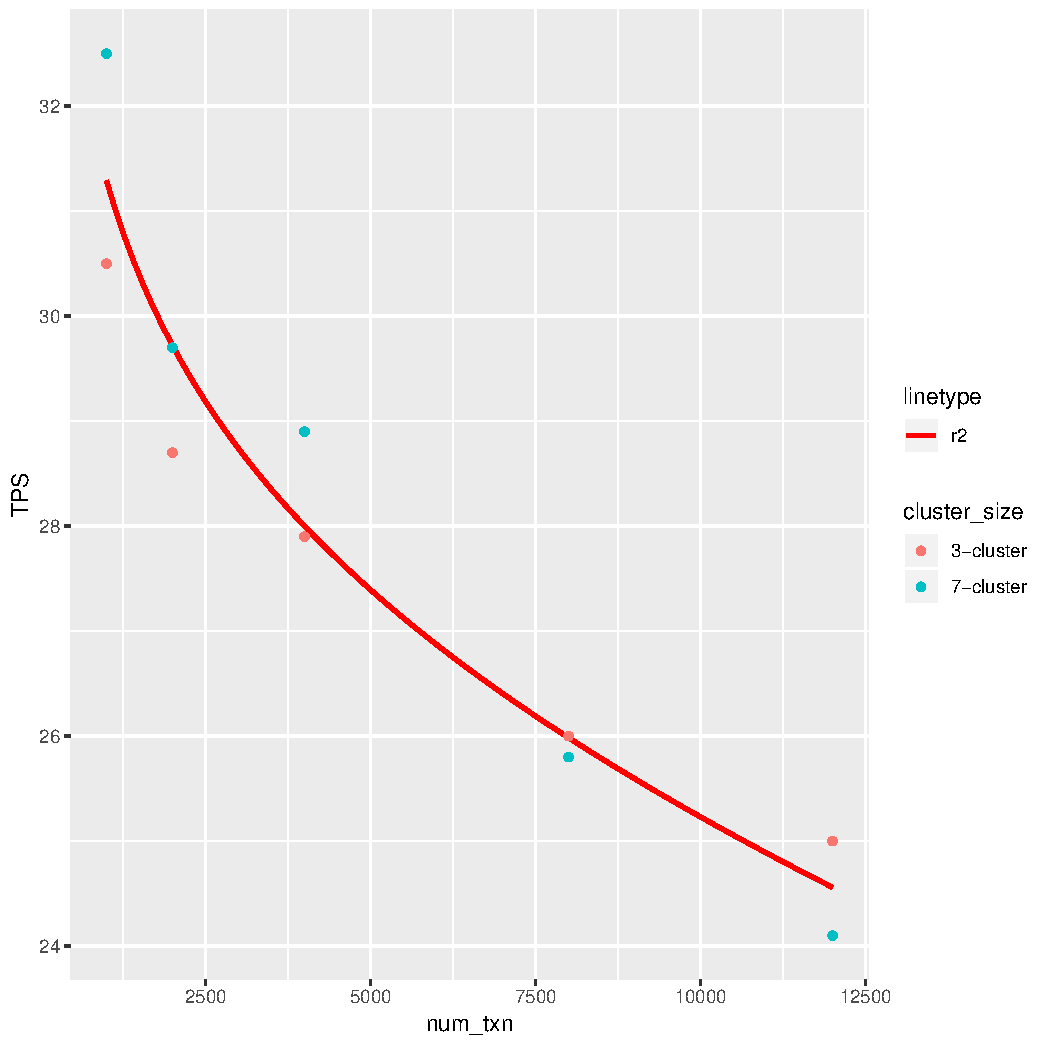
\includegraphics[width=0.45\textwidth]{figures/single_txn.pdf}
    \caption{
        Experimental results for single transaction.
     }
\label{single_txn}
\end{center}
\end{figure}



\subsubsection {Bundle transaction test}

By default, each block in StreamNet will only support one transaction. And the performance on this configuration is as Figure~\ref{single_txn} shows.

\begin{figure}[!ht]
\begin{center}
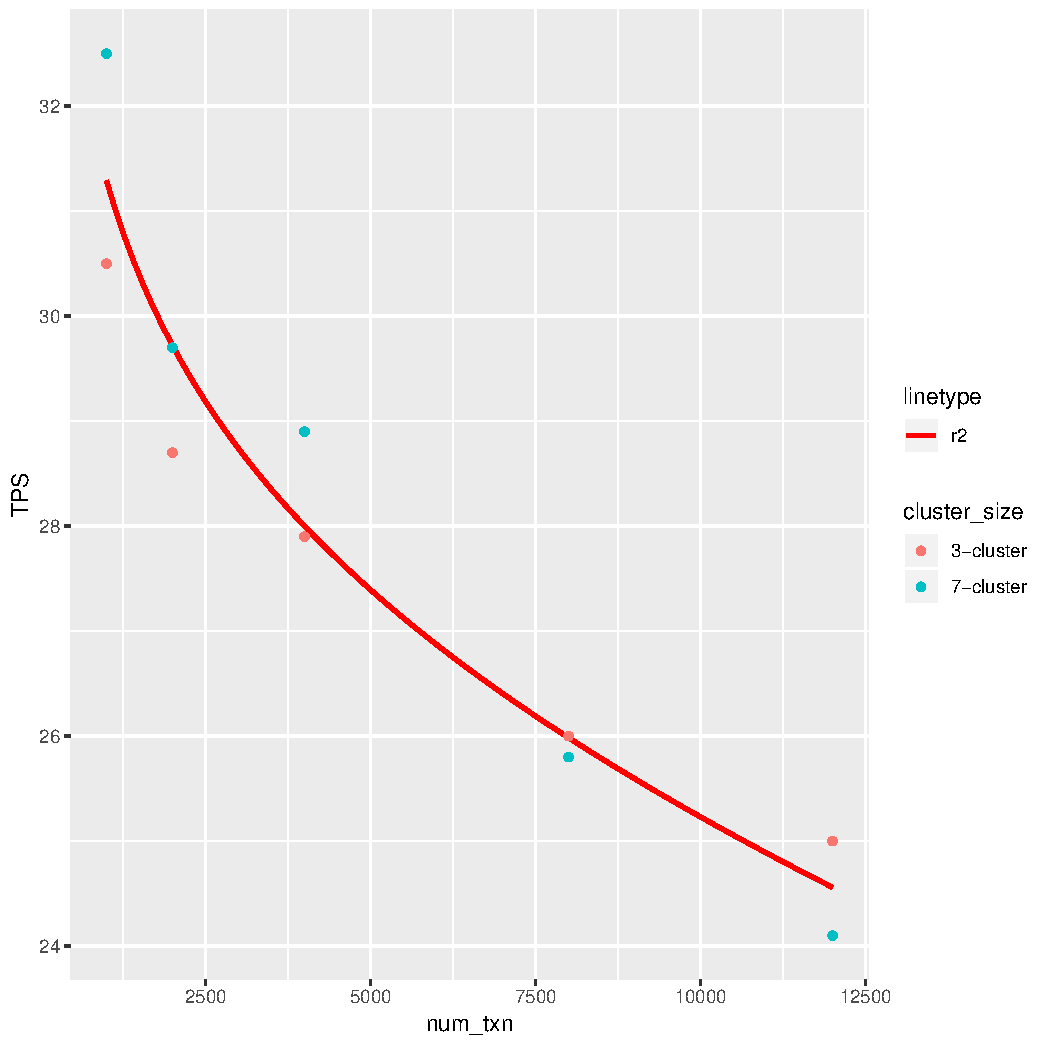
\includegraphics[width=0.45\textwidth]{figures/single_txn.pdf}
    \caption{
        Experimental results for single transaction.
     }
\label{single_txn}
\end{center}
\end{figure}


